\chapter{Синтез регулятора с заданной степенью устойчивости}
\label{ch:chap1}
\section{Условие задачи}

Рассмотреть систему:
$$
  \dot{x} = Ax + Bu
$$ и выполнить следующие шаги:

\begin{itemize}
\item   Найти собственные числа матрицы $A$ и определить управляемость каждого из них. 
Сделать вывод об управляемости и стабилизируемости системы.
\item Определить, любой ли желаемой степени устойчивости вы можете добиться от
данной системы при помощи регулятора вида $u = Kx$. Объяснить, почему, и, если не любой, то определить максимальную возможную.
\item Построить схему моделирования системы замкнутой регулятором $u = Kx$.
\item Задаться не менее, чем парой значений желаемой степени устойчивости $\alpha > 0$.
Если существуют ограничения на достижимые степени устойчивости, то одна из
выбранных $\alpha$ должна быть максимально возможной, а другие достижимыми. По
старайтесь взять достаточно отличающиеся значения $\alpha$.
\item Для каждого из выбранных значений $\alpha$ синтезировать регулятор, обеспечивающий заданную степень устойчивости, 
при помощи матричного неравенства типа Ляпунова.
  \begin{itemize}
    \item Найти соответствующую матрицу регулятора $K_1$, обеспечивающую желаемую степень устойчивости $\alpha$ \textbf{без ограничений на управление}.
    \item Найти соответствующую матрицу регулятора $K_2$, обеспечивающую желаемую степень устойчивости $\alpha$ \textbf{совместно с решением задачи минимизации управления}.
    \item  Определить собственные числа матриц замкнутых систем $(A+BK1)$ и $(A+BK2)$и сравнить с желаемой степенью устойчивости 
    в подтверждение корректности синтеза регуляторов и между собой. Сделать выводы.
    \item Выполнить компьютерное моделирование с начальными условиями системы 
    $x(0) = \begin{bmatrix} 1&1&1 \end{bmatrix}^T$. Построить  графики состояния системы $x(t)$ и управления $u(t)$. Сопоставить результаты.
  \end{itemize}
\item Для каждого из выбранных значений $\alpha$ синтезировать регулятор, обеспечивающий заданную степень устойчивости, при помощи матричного
 уравнения типа Риккати при $\nu = 2$ и $R =1$.
\begin{itemize}
  \item Найти соответствующую матрицу регулятора $K_3$, обеспечивающую желае
  мую степень устойчивости $\alpha$ при $Q = I$.
  \item Найти соответствующую матрицу регулятора $K_4$, обеспечивающую желае
  мую степень устойчивости $\alpha$ при $Q = 0$.
  \item Определитьсобственныечисламатрицзамкнутыхсистем $(A+BK_3)$ и $(A+BK_4)$
   и сравнить с желаемой степенью устойчивости в подтверждение корректности синтеза регуляторов, 
   между собой и с полученными для регуляторов с матрицами $K_1$ и $K_2$. Сделать выводы.
  \item Выполнить компьютерное моделирование с начальными условиями системы 
  $x(0) = \begin{bmatrix} 1&1&1 \end{bmatrix}^T$.  Построить  графики состояния системы $x(t)$ и управления $u(t)$. 
  Сопоставить результаты с полученными для замкнутых систем с матрицами регуляторов $K_1$ и $K_2$.
\end{itemize}
\end{itemize}

\newpage
\section{Решение задачи}

Параметры для объекта:
$$
  A = \begin{bmatrix}
  12 & -1 & 14 \\
  6 & 0 & 6 \\
  -6 & -2 & -8 
  \end{bmatrix} \tab
  B = \begin{bmatrix}
    11 \\ 7 \\ -7 
  \end{bmatrix}
$$

\subsection{Исследование управляемости системы}

Найдём собственные числа матрицы $A$:
$$
    \lambda_{1,2} = 3 \pm 3i, \tab \lambda_3 = -2
$$

Воспользуемся результатами из прошлой работы. Система будет не полностью управляемой, но стабилизируемой, всю малину испортит неуправляемое собственное число $\lambda_3 = -2$, но оно устойчивое.

\subsection{Желаемая степень устойчивости}

В нашем случае система не устойчивая, поскольку есть моды с положительной вещественной частью. Однако, модальным регулятором, 
мы можем сдвинуть все моды, кроме $\lambda_3$, поэтому если одна из сдвинутых мод будет меньше $\lambda_3$, то они и станет степенью устойчивости, в противном случае
степень устойчивости после замыкания регулятором станет $\lambda_3 = -2$. 

\subsection{Первая желаемая степень устойчивости}
$$
    \alpha_1 = 2
$$

Для такой степени устойчивости (максимальной) синтезируем регулятор при помощи \textbf{матричного неравенства Ляпунова}:
$$
  PA^T + AP + 2\alpha P + Y^TB^T \preceq 0, \tab P \succ 0, \tab K=YP^{-1}
$$

Решим уравнения и получим $K_1$, обеспечивающую заданную степень устойчивости \textbf{без ограничений на управление}:
$$
  K_1 = \begin{bmatrix}
    10.06 & -8.83 & 9.25
  \end{bmatrix}, \tab\rightarrow\tab \sigma(A+BK_1)=\{ -4.94 \pm 7.77i, -2 \}
$$

Чтобы получить вторую матрицу регулятора $K_2$, которая ещё и решает \textbf{задачу минимизации управления}, нам потребуется указать дополнительные условия к уравнению выше:
$$
  \begin{bmatrix}
    P & x_0 \\
    x_0^T & 1
  \end{bmatrix} \succ 0, \tab
  \begin{bmatrix}
    P & Y^T \\
    Y &\mu^2I
  \end{bmatrix} \succ 0, \tab \rightarrow \tab 
  K_2 = \begin{bmatrix}
    4 & -4.17 & 3.65
  \end{bmatrix}
$$ Тогда регулятор  $K = YP^{-1}$ будет гарантировать $||u(t)|| \leq \mu$ при $x(0)=x_0$.
Собственные числа в таком случае:
$$
  \sigma(A+BK_2)=\{ -2.37 \pm 5.25i, -2 \}
$$

Как можно заметить, управляемые собственные числа в обеих случаях у синтезированного регулятор не превышают заданное $\alpha_1$ по модулю, 
а также в случае с ограниченным управлением стали несколько меньше, что говорит о том, что ограничение на управление подействовало на моды напрямую, 
синтез корректен и мы продемонстрируем это моделированием:



\begin{figure}[ht]
  \centering
  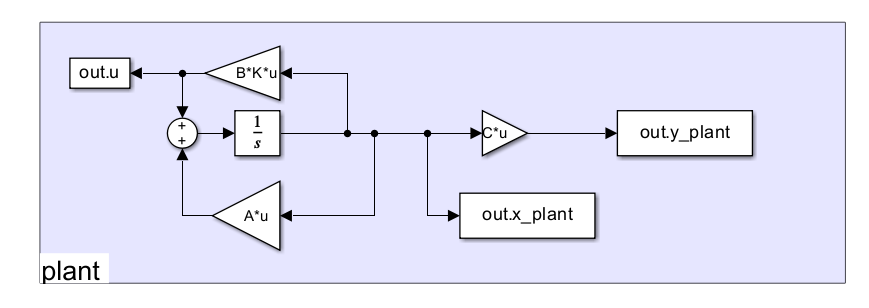
\includegraphics[width=1.0\textwidth]{model_controller.png}
  \caption{Модель с модальным регулятором}
\end{figure}


С помощью неё построим графики управления $u(t)$ от регулятора и вектора состояния замкнутой системы $x(t)$
при начальных условиях $x(0) = \begin{bmatrix} 1 & 1 & 1 \end{bmatrix}^T$:
\newpage
\begin{figure}[ht]
  \centering
  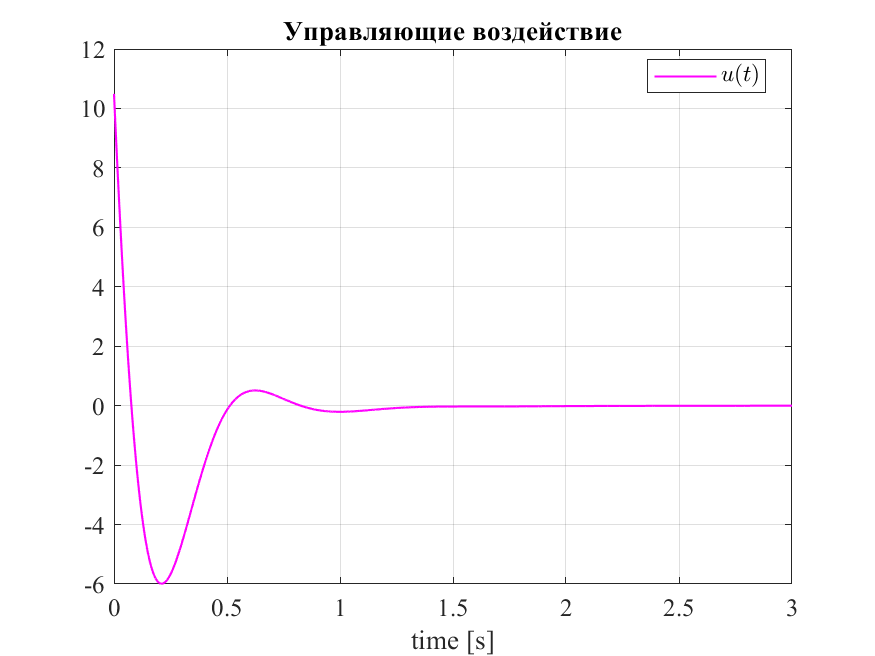
\includegraphics[width=0.8\textwidth]{ctrl1_u1.png}
  \caption{Сигнал управления, регулятор $K_1$}
\end{figure}
\begin{figure}[ht]
  \centering
  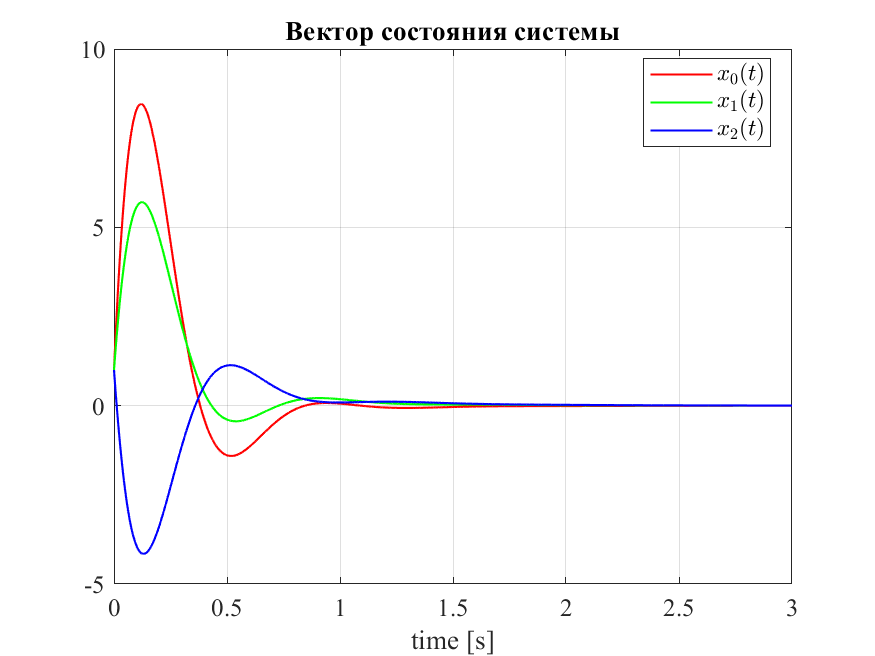
\includegraphics[width=0.8\textwidth]{ctrl1_x1.png}
  \caption{Состояние системы, регулятор $K_1$}
\end{figure}
\newpage
\begin{figure}[ht]
  \centering
  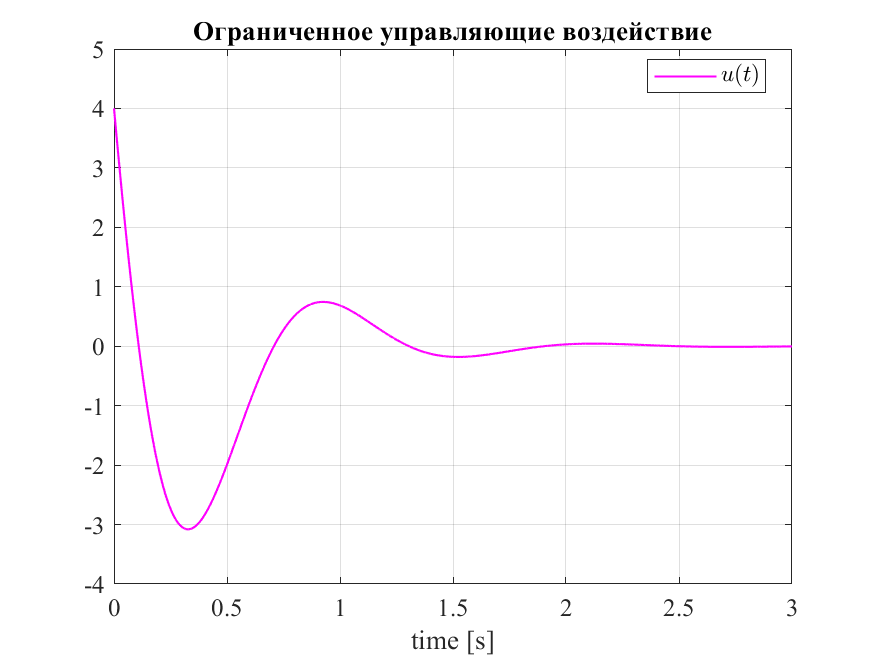
\includegraphics[width=0.8\textwidth]{ctrl1_u2.png}
  \caption{Сигнал управления, ограниченный регулятор $K_2$}
\end{figure}
\begin{figure}[ht]
  \centering
  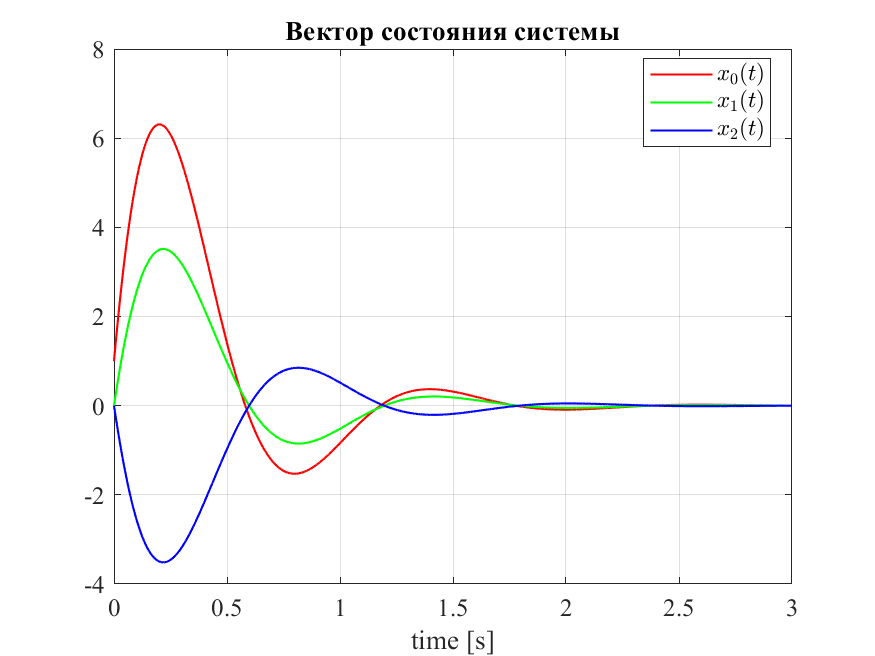
\includegraphics[width=0.8\textwidth]{ctrl1_x2.png}
  \caption{Состояние системы, ограниченный регулятор $K_2$}
\end{figure}

Как можно заметить - ограничением управления немного увеличили время переходного процесса и перерегулирование, но взамен мы возможно не перегрели обмотки двигателя.

Дополнительно синтезируем регулятор другим методов, при помощи \textbf{матричного уравнения типа Риккати} при $\nu=2, R=1$:
$$
  A^TP + PA + Q - \nu PBR^{-1}B^T P + 2\alpha P =0, \tab P \succ 0, \tab K=-R^{-1}B^TP
$$

Найдём матрицы регуляторов $K_3, K_4$ при $Q = I, Q = 0$:
$$
  K_3 = \begin{bmatrix}
      7.18 & -5.98 & 7.1
    \end{bmatrix}, \tab
  K_4 = \begin{bmatrix}
    4.26 & -3.86 & 4.26
  \end{bmatrix}
$$
$$
  \sigma(A+BK_3)=\{ -3.58 \pm 6.94i, -2 \}, \tab \sigma(A+BK_4)=\{ -2 \pm 5.83i, -2 \}
$$
Матричное уравнение Риккати, - частный случай $LMI$ Ляпунова, поэтому это уравнение лишь даёт одно конкретное решение из области неравенства,
поэтому в целом $K_1, K_2$ и $K_3, K_4$ матрицы схожи, и поведение системы также. 
Однако бОльшие различия можно заметить, сравнив $K_3, K_4$ между собой: при нулевой $Q$ мы позволяем вектору состояния иметь больших размах, перерегулирование, потому что убираем
"штраф на вектор состояния". Это можно заметить на графиках моделирования:

\begin{figure}[ht]
  \centering
  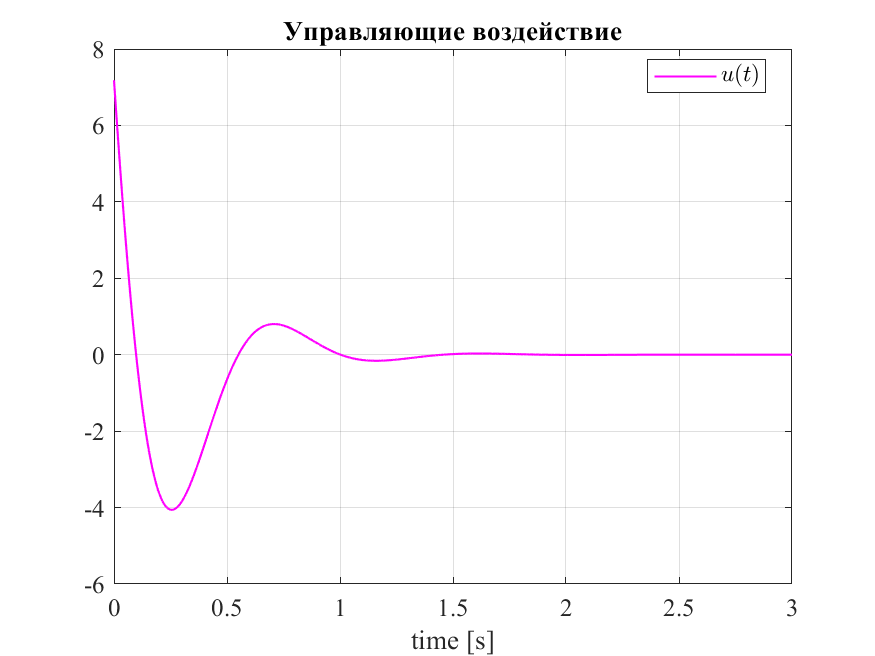
\includegraphics[width=0.8\textwidth]{ctrl1_u5.png}
  \caption{Сигнал управления, $Q=I$}
\end{figure}
\newpage
\begin{figure}[ht]
  \centering
  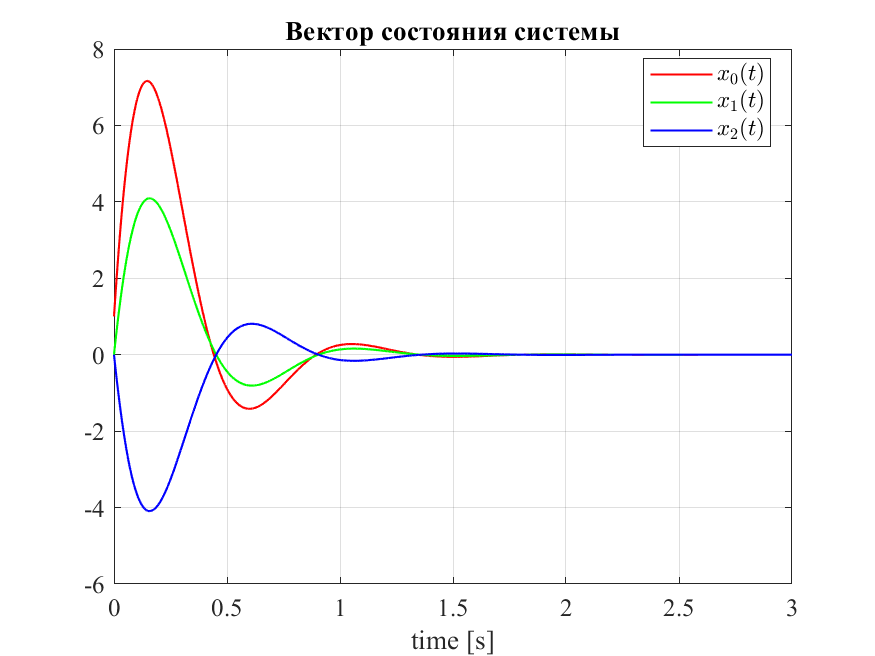
\includegraphics[width=0.8\textwidth]{ctrl1_x5.png}
  \caption{Состояние системы, $Q=I$}
\end{figure}
\begin{figure}[ht]
  \centering
  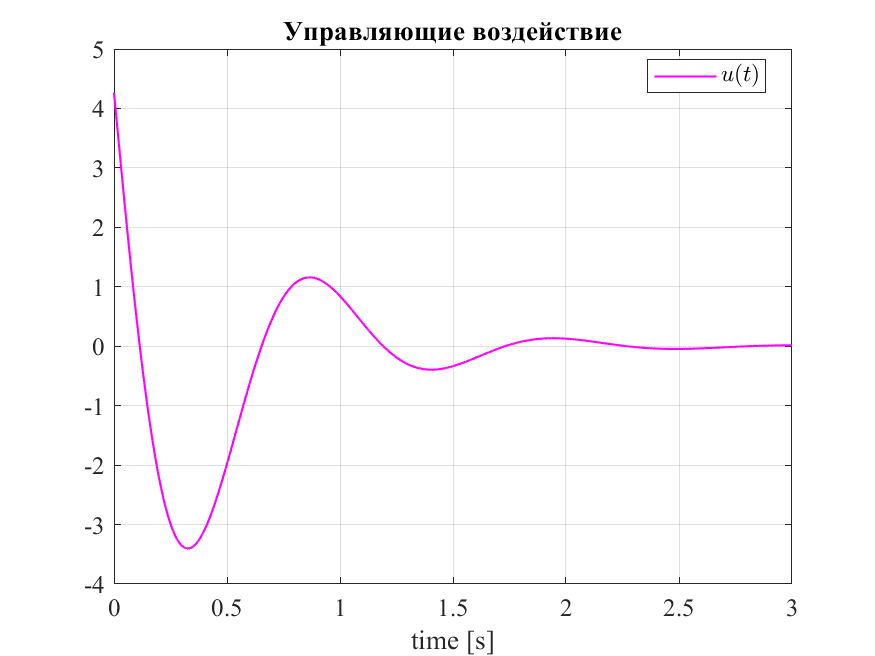
\includegraphics[width=0.8\textwidth]{ctrl1_u7.png}
  \caption{Сигнал управления, $Q=0$}
\end{figure}
\newpage
\begin{figure}[ht]
  \centering
  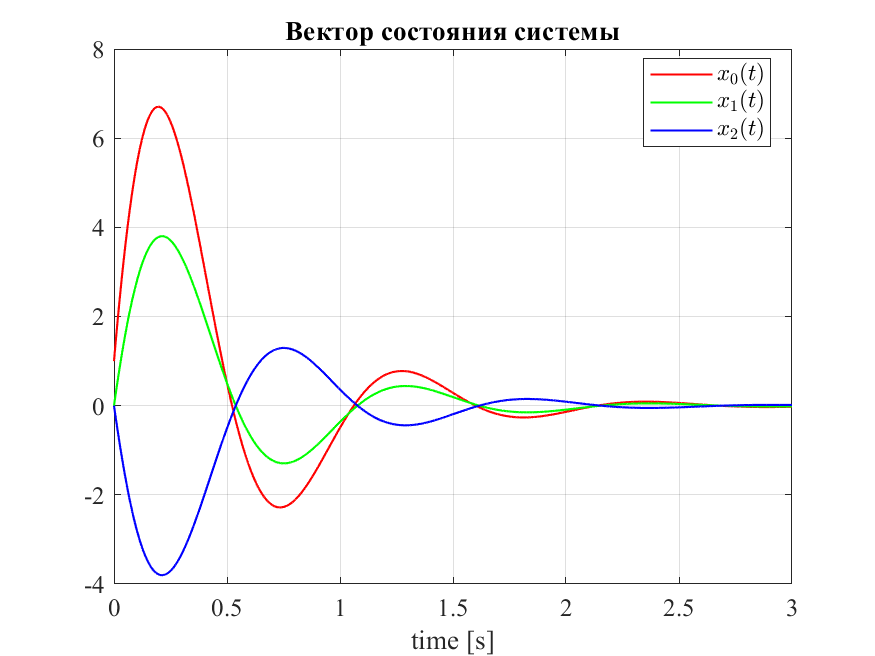
\includegraphics[width=0.8\textwidth]{ctrl1_x7.png}
  \caption{Состояние системы, $Q=0$}
\end{figure}

\newpage
\subsection{Вторая желаемая степень устойчивости}
$$
    \alpha_2 = 0.5
$$

Синтезируем регулятор при помощи \textbf{матричного неравенства Ляпунова}, без ограничений на управление и с ним:
$$
  K_1 = \begin{bmatrix}
      6.64 & -6.31 & 6.27
    \end{bmatrix}, \tab
  K_2 = \begin{bmatrix}
    1.75 & -2.38 & 1.51
  \end{bmatrix}
$$
$$
  \sigma(A+BK_1)=\{ -4.5 \pm 5.5i, -2 \}, \tab \sigma(A+BK_2)=\{ -1.03 \pm 3.86i, -2 \}
$$

Как можно заметить, управляемые собственные числа в обеих случаях у  регулятора не превышают заданное $\alpha_2$ по модулю, 
а также в случае с ограниченным управлением стали несколько меньше, что говорит о том, что ограничение на управление подействовало на моды напрямую, 
синтез корректен и мы продемонстрируем это моделированием:

\newpage
\begin{figure}[ht]
  \centering
  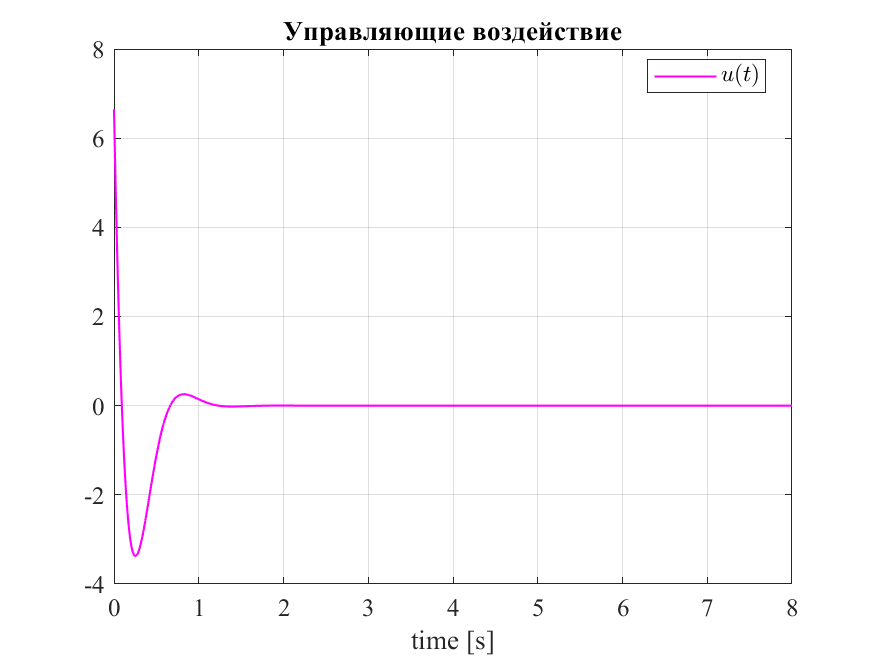
\includegraphics[width=0.8\textwidth]{ctrl1_u3.png}
  \caption{Сигнал управления, регулятор $K_1$}
\end{figure}
\begin{figure}[ht]
  \centering
  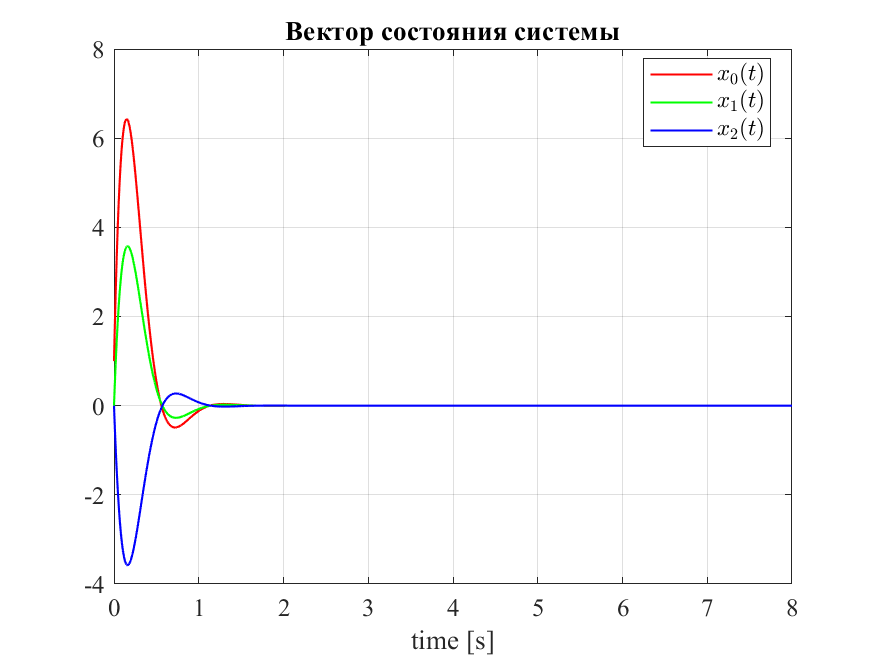
\includegraphics[width=0.8\textwidth]{ctrl1_x3.png}
  \caption{Состояние системы, регулятор $K_1$}
\end{figure}
\newpage
\begin{figure}[ht]
  \centering
  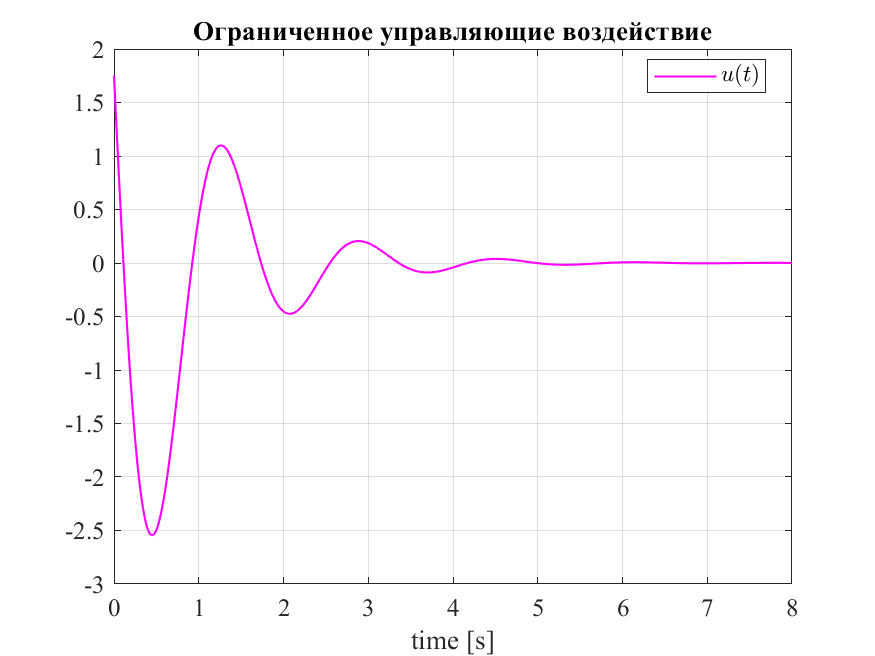
\includegraphics[width=0.8\textwidth]{ctrl1_u4.png}
  \caption{Сигнал управления, ограниченный регулятор $K_2$}
\end{figure}
\begin{figure}[ht]
  \centering
  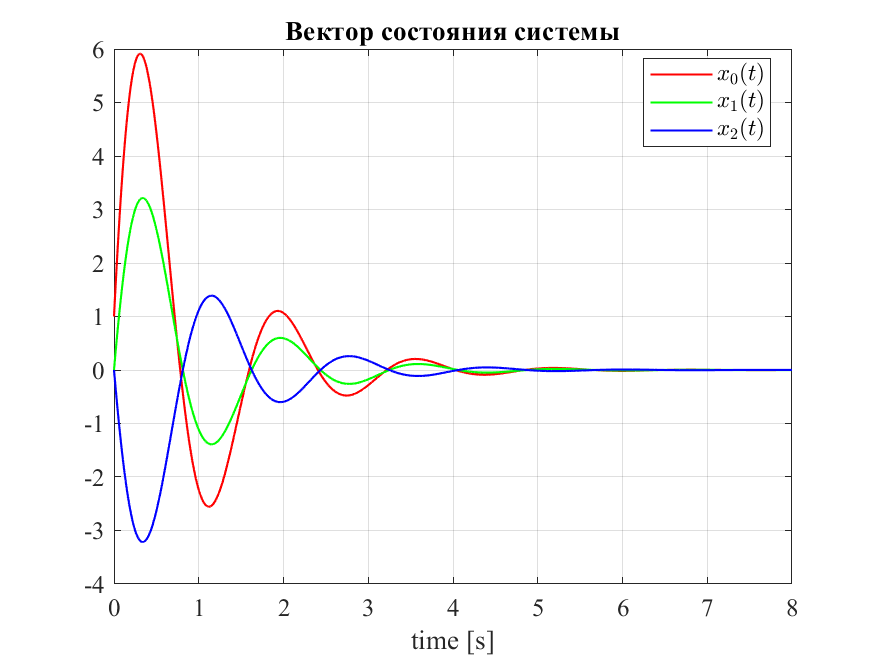
\includegraphics[width=0.8\textwidth]{ctrl1_x4.png}
  \caption{Состояние системы, ограниченный регулятор $K_2$}
\end{figure}

Как и с прошлым параметром $\alpha$ - ограничением управления немного увеличили время переходного процесса и перерегулирование, 
однако сейчас мы значительно увеличили время переходного процесса, потому что взяли $\alpha_2 < \alpha_1$.

Дополнительно синтезируем регулятор другим методов, при помощи \textbf{матричного уравнения типа Риккати} при $\nu=2, R=1$:

Найдём матрицы регуляторов $K_3, K_4$ при $Q = I, Q = 0$:
$$
  K_3 = \begin{bmatrix}
    4.44 &  -4.07 & 4.44
    \end{bmatrix}, \tab
  K_4 = \begin{bmatrix}
   2.0 & -2.14 & 2.0
  \end{bmatrix}
$$
$$
  \sigma(A+BK_3)=\{ -2.35 \pm 5.7i, -2 \}, \tab \sigma(A+BK_4)=\{ -0.5 \pm 4.6i, -2 \}
$$

Матричное уравнение Риккати, - частный случай $LMI$ Ляпунова, поэтому это уравнение лишь даёт одно конкретное решение из области неравенства,
поэтому в целом $K_1, K_2$ и $K_3, K_4$ матрицы схожи, и поведение системы также. 

Здесь различия в отсутствии/наличии штрафа на вектор состояния в виде $Q$ также ещё проще заметить, ведь мы выбрали скорость сходимости значительно меньше,
поэтому при отсутствии штрафа система позволила вектору состояния бОльшее перерегулирование, это заметно на графиках моделирования:

\begin{figure}[ht]
  \centering
  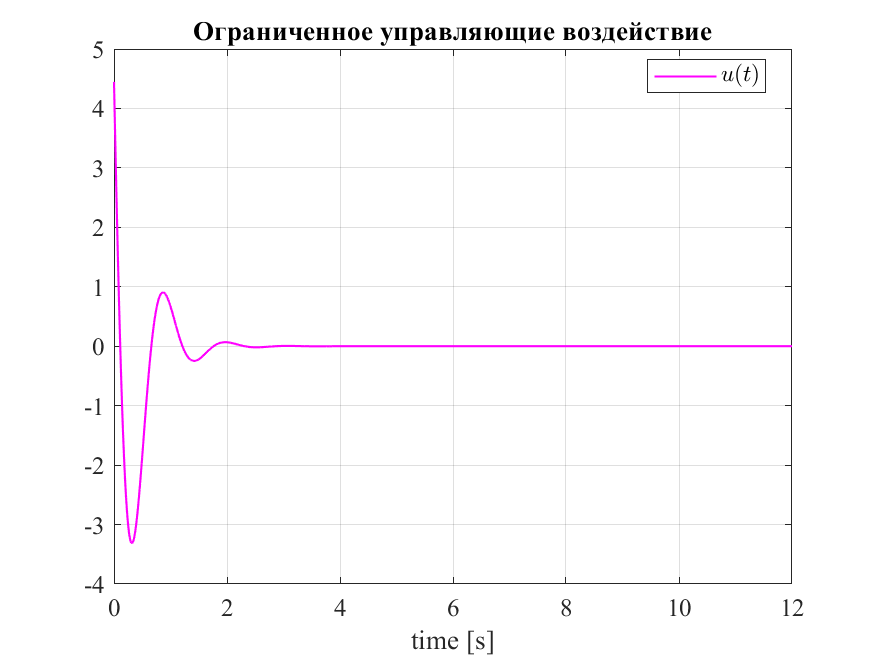
\includegraphics[width=0.8\textwidth]{ctrl1_u6.png}
  \caption{Сигнал управления, $Q=I$}
\end{figure}
\newpage
\begin{figure}[ht]
  \centering
  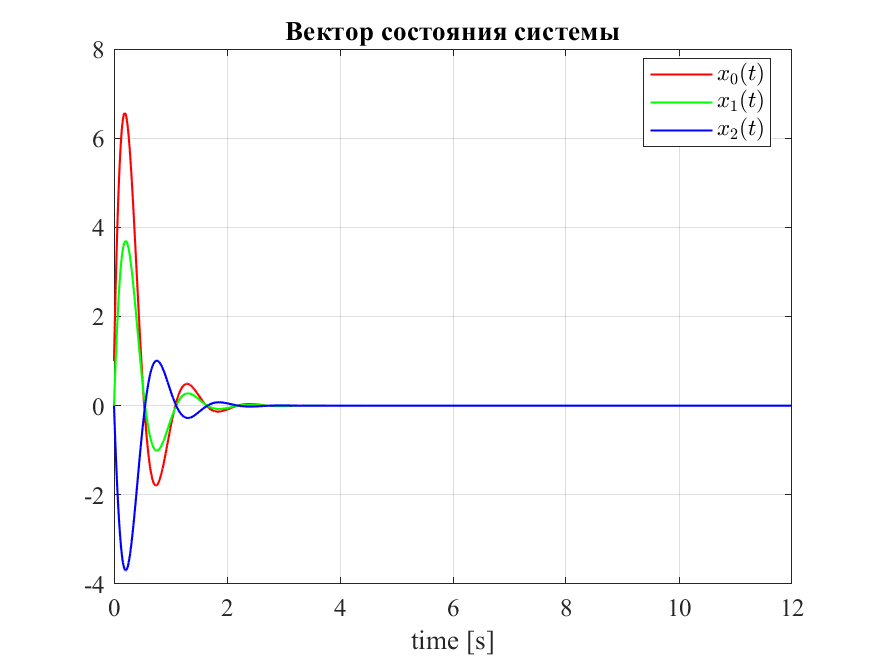
\includegraphics[width=0.8\textwidth]{ctrl1_x6.png}
  \caption{Состояние системы, $Q=I$}
\end{figure}
\begin{figure}[ht]
  \centering
  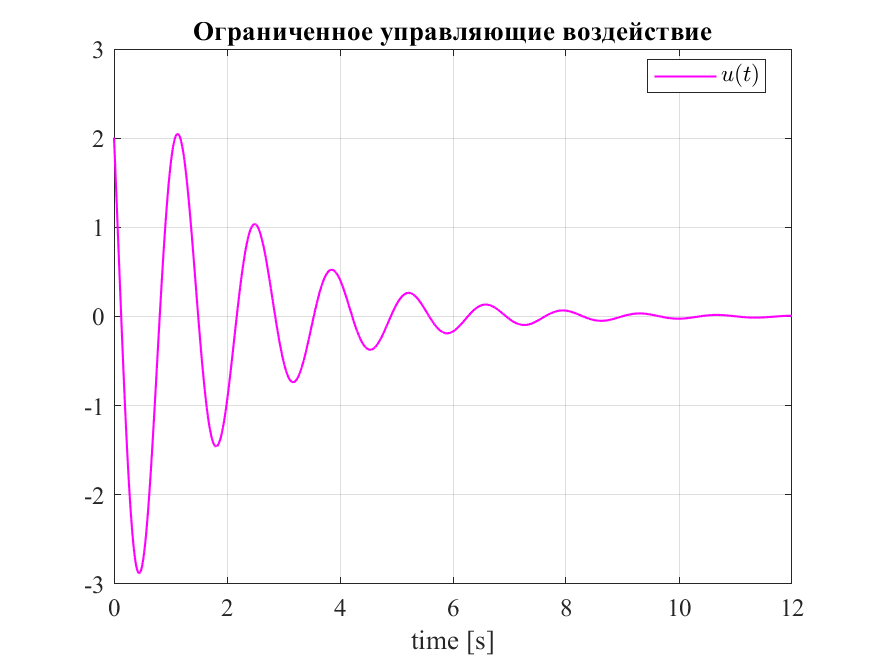
\includegraphics[width=0.8\textwidth]{ctrl1_u8.png}
  \caption{Сигнал управления, $Q=0$}
\end{figure}
\newpage
\begin{figure}[ht]
  \centering
  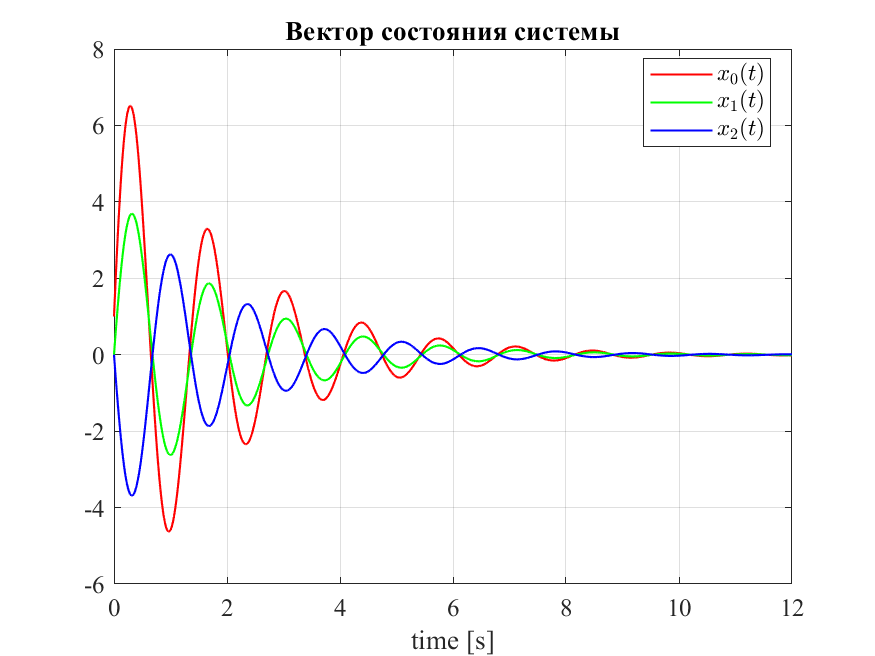
\includegraphics[width=0.8\textwidth]{ctrl1_x8.png}
  \caption{Состояние системы, $Q=0$}
\end{figure}

\subsection{Вывод}

В этом задании мы синтезировали регулятор с заданной степень устойчивости для стабилизируемой системы, для этого пришлось применить метод усечения, чтобы работать только с управляемой частью.
Для вычисления матриц коэффцициентов мы воспользовались двумя способами - решением матричного неравенства типа Ляпунова, а также матричным уравнением Риккати. 
Оба способа показали спектры матрицы $(A+BK)$ не меньше чем заданный параметр $\alpha$ (скорость сходимости), что свидетельствует о корректном синтезе.

\endinput